\documentclass[../main.tex]{subfiles}
\begin{document}

\section{Neural networks}
The brain is considered the most complex system that we know, composed of approximately $9\cdot10^{10}$ neurons, each projecting signals to thousands of other neurons \citep{Vreeken2003SpikingNN,https://doi.org/10.1002/cne.21974}.
Unraveling the complexity of such a vast neural network necessitates sophisticated measurement methods.
Traditional non-invasive approaches, such as \textbf{functional magnetic resonance imaging} (fMRI), \textbf{electroencephalography} (EEG) and \textbf{magnetoencephalography} (MEG), provide valuable insights into overall brain activity.
However, they come with limitations, either in accessing information on deeper brain structures or exhibiting poor temporal resolution.
To gain insights into deep brain structures, intra-cranial recordings and the measurement of the \textbf{local field potential} offer valuable avenues \citep{buzsaki2012origin}.
 
Electrical extracellular recordings have been a main research topic in electrophysiology for almost a century.
The high-frequency part of these signals (>500 Hz), \textit{i.e.}, the multi-unit
activity (MUA), contains information about the firing of action potentials in surrounding neurons \citep{buzsaki_large-scale_2004}. 
In contrast, the low-frequency part, the so-called local field potential (LFP), contains information about how those neurons integrate synaptic inputs \citep{leski_frequency_2013}.
The interpretation of LFPs is ambiguous and difficult since extracellular signals arise from multiple neural processes.
The biggest consensus is that the main component of the extracellular potential arises from the transmembrane currents of the neurons near the recording electrode (hundreds of millimeters). 
However, more elements are involved in the generation of LFPs, such as the morphological characteristics of contributing cells, synaptic positioning, the level of correlation of synaptic inputs, and sodium and calcium spikes, among others \citep{buzsaki_origin_2012}.
%One major contribution of computational neuroscience to the study of LFPs is the development of biophysical models that simulate the electrical activity of neural populations.
%These models incorporate the morphological and biophysical properties of individual neurons and their connectivity patterns to simulate the emergent dynamics of LFPs.
%By integrating experimental data with computational models, researchers can gain insights into how specific cell and network properties shape the observed LFP patterns.
\subsection{Local field potential}
The methodology used for estimating LFPs within neural network models frequently varies based on the specific type of neural model used.
When networks consider point-like neurons, as discussed in the previous section, a common method is to characterize LFPs as the averaged membrane potential of the network \citep{palmigiano_flexible_2017-1}.
However, alternative approaches have been proposed, showcasing the versatility of capturing neural dynamics.
Some of them are methods based on the network firing rate \citep{buehlmann_neuronal_2008}, a convolution-based version \citep{telenczuk_kernel-based_2020}, or the summation of all synaptic currents \citep{mazzoni_encoding_2008, negahbani_neuroimage_2018}.
The choice of using point-like neurons in these models is often motivated by considerations of computational efficiency. 
This simplification entails omitting details related to neuronal morphology and dendritic dynamics, among other properties, to facilitate large-scale simulations and analyses.

In contrast, multicompartment neuron models are designed to capture individual neurons' intricate anatomical and biophysical properties, including dendrites, soma, and axons, making a more realistic estimation.
Each compartment of a neuron contributes differently to the extracellular field potential, and consequently, the LFP has to be estimated by adding these contributions.
Figure \ref{fig:LFP-measurement} illustrates the conceptualization of this process, highlighting the distinctive contributions of different neuronal compartments to the overall LFP.
This detailed modelling approach is crucial to capture the spatial and temporal complexities inherent in neural network dynamics.
This offers a more nuanced understanding of how individual components contribute to the observed extracellular field potentials.
In the most general scenario, obtaining the formula that describes the contribution of activity in a multicompartment neural network model to extracellular potential consists of finding a solution to the \textbf{Laplace equation}:
\begin{equation}
    \nabla^2\Phi = 0
    \label{eq:laplace-equation},
\end{equation}
where $\Phi$ is the extracellular potential.
Some approximations and conditions are assumed: the quasistatic approximation of Maxwell's equations, in which the electric and magnetic fields are decoupled, and the assumption of an infinite volume conductor in which electrical conductivity $\sigma$ is ohmic, frequency-independent, homogeneous, and isotropic \citep{einevoll_modelling_2013}.
\begin{enumerate}
\item \textbf{Point source approximation} \citep{holt_electrical_1999}.
The description of the LFP is given by Culomb's law as the solution of \eqref{eq:laplace-equation}:
\begin{equation}
    \Phi(\mathbf{r},t) = \sum_{i=1}^{n_s}\displaystyle\frac{I_i(t)}{4\pi\sigma r_i}, 
    \label{eq:point-source-approximation}
\end{equation}
where $n_s$ is the number of current sources (compartments), $r_i$ is the distance between the electrode and the $i$-th current source, $\sigma$ is the extracellular conductivity, and $I_i(t)$ is the transmembrane current, which consists of the sum of the total ionic currents and the capacitive currents:
\begin{equation}
    I_\text{transmembrane} = I_\text{ionic} + c_m\displaystyle\frac{\partial v}{\partial t}.
    \label{eq:transmembrane-current}
\end{equation}
\item \textbf{Line source approximation} \cite{gold_origin_2006}.
This approximation assumes locating the net transmembrane current for each compartment on a line down its center.
Assuming a linear distribution of currents in equation \eqref{eq:laplace-equation}, the extracellular potential, in cylindrical coordinates, is given by:
\begin{equation}
    \begin{aligned}
        \Phi(\mathbf{h},t) &= \sum_{i=1}^{n_s} \frac{1}{4\pi \sigma}\int_{-\Delta s_i}^{0}\displaystyle\frac{I_i(t) ds}{\Delta s_i\sqrt{r_i^2+(h_i-s_i)^2}} \\
        \quad &  = \sum_{i=1}^{n_s} \frac{I_i(t)}{4\pi \sigma\Delta s_i} \log \Bigg( \displaystyle\frac{\sqrt{h_i^2+r_i^2}-h_i}{\sqrt{l_i^2+r_i^2}-l_i} \Bigg), 
    \end{aligned}
        \label{eq:line-source-approximation}
    \end{equation}
where $r_i$ is the radial distance from the compartment, $h_i$ is the longitudinal distance from the end of the compartment and $l = \Delta s_i + h_i$ is the distance from the beginning of the compartment. 
This implementation has been known to better approximate the extracellular signal, except at a very close distance, less than 1 $\mu$m away from the measurement point.

\item \textbf{Low pass filtering approximation} \citep{bedard_modeling_2004}.
In the two previous approximations, the assumption of homogeneous media led to a constant spatial and temporal conductivity.
However, in situations where this assumption is invalid, giving rise to spatially varying conductivity (non-homogeneous media), the continuity equation determines a time-dependent density charge.
Without delving into intricate details, this results in the media exhibiting characteristics analogous to those of a low-pass filter.
In this scenario, the extracellular potential is described by:
\begin{equation}
    \Phi = \sum_{i=1}^{n_\text{sources}}I_i \exp\Big(-\displaystyle\frac{t_i}{RC} \Big),
     \label{eq:low-pass-approximation}
\end{equation}
where $t_i$ is the time it takes the \textit{field} from the source to arrive at the measuring point ($r_i/v$, where $v$ is the propagation velocity), and $R$ and $C$ are the resistance and the capacitance of the extracellular medium, respectively.
\end{enumerate}
\begin{figure}[!htb]
    \centering
    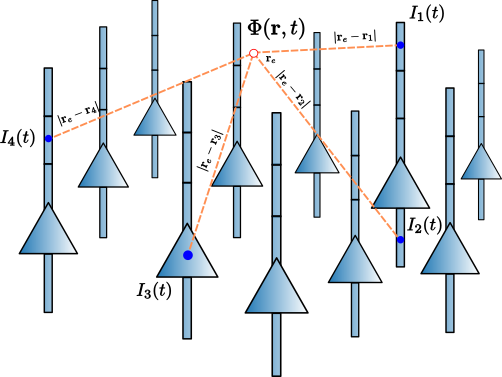
\includegraphics[width=0.8\textwidth]{chapter1/figures/LFP-schematics-2.png}
    \caption{\textbf{LFP computation}.
    Biophysical scheme to compute LFP in a network of multicompartmental pyramidal neurons.
    The contribution of each compartment depends on the reletaive distance to $\mathbf{r_e}$, the position where the electrode is placed.}
    \label{fig:LFP-measurement}
\end{figure}
\subsection{Neural population models}
Developing a neural network to model a specific brain region, or even the entire brain, presents a substantial challenge, particularly in terms of computational time.
To address this challenge, alternative models incorporating populations of neurons have been developed.
The so-called \textbf{neural mass models} serve as pragmatic solutions to mitigate the computational costs associated with simulating large-scale neural networks.
These models are designed to characterize the collective behavior of a substantial population of neurons within the brain as a singular entity, reducing the intricate dynamics of neural networks by focusing on the aggregate activity of a neuronal group \citep{deschle_directed_2019}.
%%%%%%%%%%%%%%%%%%%%%%%%%%%%%%%%%%%%%%
Considering neural mass models as building blocks, network connectivity-based approaches have been instrumental in unraveling the complexities of large-scale brain function \citep{10.3389/fams.2023.1128224,deco_key_2009, honey_network_2007}.
These studies explore the emergence of functional connectivity networks, elucidating dynamic patterns of temporal coherence of activity between different brain regions.
%%%%%%%%%%%%%%%%%%%%%%%%%%%%%%%%%%%%%%%
Some of the most recognized models are the \textbf{Wilson-Cowan model} \citep{wilson1973mathematical}, the \textbf{Jansen-Rit model} \citep{jansen1995electroencephalogram}, the \textbf{Wendling model} \cite{wendling2002epileptic} and the \textbf{Grimbert model} \citep{grimbert2006bifurcation}.

One of the most intriguing and fundamental phenomena that emerges from the intricate interaction between neurons and the population of neurons is \textbf{synchronization}.
A key model that has played a pivotal role in unraveling this intricate phenomenon is the \textbf{Kuramoto model} \citep{kuramoto1975international,kuramoto1984chemical}.
Introduced by Yoshiki Kuramoto in 1984, this model was developed to characterize the behavior of oscillatory biological and chemical systems.
However, it became a widespread tool in many fields, including neuroscience, due to its versatile applicability and robust theoretical foundation.
The \textbf{Kuramoto model} provides a robust framework for investigating synchronization patterns within coupled oscillatory systems, proving particularly adept at elucidating emergent phenomena in neural populations \citep{strogatz2000kuramoto,acebron2005kuramoto}.
%%%%%%%%%%%%%%%%%%%%%%%%%%%%%%%%%%%%%%%
By condensing the intricate dynamics of the brain into phase interactions, wherein the dynamics of a neural population is reduced to a phase oscillator, this model provides valuable insights into the emergent synchrony patterns observed in large-scale brain networks.
In contrast to more intricate neural network models, the Kuramoto model operates at a higher level of abstraction, facilitating efficient exploration of the influence of coupling strength and network topology on the emergence of synchronous patterns \citep{bick2020understanding,strogatz2000kuramoto,acebron2005kuramoto}.

%%%%%%%%%%%%%%%%%%%%%%%%%%%%%%%%%%%%%%%%%%%
The model consists of a population of $N$ coupled phase oscillators $\theta_i(t)$ each possessing natural frequencies $\omega_{i,0}$ distributed according to a given probability density function $g(\omega)$, and whose dynamics are governed by: 
\begin{equation}
    \displaystyle\frac{d}{dt}\theta_i(t) = \omega_{i,0} + \displaystyle\sum_{j=1}^{N}K_{ij}\sin\big(\theta_j(t)-\theta_i(t) \big),
    \label{eq:kuramoto}
\end{equation}
where $\omega_{i,0}$ is the intrinsic frequency of the $i$-th oscillator and $K_{ij}$ is the coupling matrix that defines the weighted connectivity pattern among the oscillators.
When the coupling is sufficiently weak, the oscillators run incoherently, whereas, beyond a certain threshold, collective synchronization emerges spontaneously.
Many different models for the coupling matrix $K_{ij}$ have been considered, such as nearest-neighbor coupling, hierarchical coupling, random long-range coupling, etc. \citep{acebron2005kuramoto}.
This model allows us to explore how coupling strength and network topology influence the emergence of synchronous patterns, shedding light on the collective dynamics of neural populations.
Importantly, the \textbf{Kuramoto model} serves as a computationally efficient abstraction, bridging the gap between theoretical insights and the complexities of simulating large-scale neural networks.

In the Chapter I, we will delve further into the concept of \textbf{synchronization} and the application of the \textbf{Kuramoto model} in the context of dimensionality reduction.
\end{document}

% Furthermore, computational techniques have facilitated the exploration of causal relationships between LFPs and behavior through closed-loop experiments. Closed-loop systems use real-time LFP recordings to inform and modulate the stimulation of specific brain regions or neural populations. By manipulating LFP activity and observing resulting behavioral changes, researchers can gain insights into the causal roles of LFP oscillations in cognitive functions and behaviors.

% In conclusion, computational neuroscience has significantly contributed to our understanding of LFPs by providing valuable tools and approaches for data analysis, modeling, and simulation. By leveraging computational techniques, researchers have unraveled the complex mechanisms underlying LFP generation, identified spectral properties, explored relationships with other neuroimaging modalities, investigated cognitive processes and neurological disorders, and even established causal links between LFPs and behavior. These advancements have paved the way for a deeper understanding of brain function and dysfunction, opening new avenues for therapeutic interventions and clinical applications.

Addtionally, different class of models are neural mass models (Jansen and Rit, 1995; Wendling et al., 2000; David and Friston, 2003; Rodrigues et al., 2010), where LFPs are estimated either through sums  of excitatory postsynaptic potentials (EPSP) (David and Friston, 2003) or of excitatory postsynaptic currents (EPSC) (Mazzoni et al., 2008).

% In addition, computational methods have facilitated the investigation of the relationship between LFPs and other neuroimaging modalities, such as electroencephalography (EEG) and functional magnetic resonance imaging (fMRI).
Integrating LFP data with these techniques allows for a more comprehensive understanding of brain dynamics and the mapping of LFP oscillations to specific brain regions and networks. Computational models have been developed to interpret and integrate these multimodal datasets, offering insights into the large-scale interactions and information flow within the brain.

Moreover, computational approaches have been instrumental in unraveling the role of LFPs in various cognitive processes and neurological disorders. 
hrough the use of network models, researchers have investigated how LFP oscillations contribute to information processing, sensory perception, attention, memory, and motor control.
Computational studies have also shed light on how abnormal LFP patterns are associated with neurological conditions, including epilepsy, Parkinson's disease, and schizophrenia.
These findings have important implications for the development of therapeutic interventions and the understanding of brain disorders.

In general, mean field models of neural activity can be divided into two classes: neural mass and neural field models. The main difference between these classes is that field models prescribe how a quantity characterizing neural activity (such as average depolarization of a neural population) evolves over both space and time as opposed to mass models, which characterize activity over time only; by assuming that all neurons in a population are located at (approximately) the same point. 
(Neural masses and fields: modeling the dynamics of brain activity)

Here we consider, in particular, how DCM treats ensemble neuronal activity as a point process (neural mass models) or explicitly incorporate a spatial dimension (neural field models). Both types describe so-called “mesoscopic” properties of neural activity, employing statistical mechanics to transform single unit activity into population activity—where appropriate composites can be used to generate macroscopic data. Since this mesoscale is hidden from direct observation, we demonstrate how these models rely upon and exploit knowledge about synaptic and cell physiology, as well as neuroanatomy.
(Neural masses and fields in dynamic causal modeling)

This use of neural fields, was proposed as a semi-quantitative treatment of electromagnetic brain activity by Jirsa and Haken (1996, 1997) and Robinson (2006).

%%%%

However, to delve deeper into the intricate orchestra of neuronal communication, researchers turn to the Local Field Potential (LFP), a valuable tool that unveils emergent properties within neural networks. The LFP provides a window into the collective behavior of neurons, capturing the synchronized electrical activity of nearby neural populations. This introduction sets the stage for exploring the nuanced emergent phenomena that characterize the dynamic interplay of neurons in the quest to understand the brain's complexities

Although much work has focused on studying large-scale networks and using mathematical models to reduce their vast dimensionality and achieve realistic dynamics of biological networks, the computational power needed hinders the simulation of networks with detailed biological features at the brain scale.

As our understanding of neural interactions deepens, the focus broadens to neural networks, which capture the collective behavior arising from interconnected neurons.
Neural networks emulate the brain's ability to process information through interconnected nodes, mimicking the synaptic connections that give rise to complex information processing and learning.